\documentclass[preprint,12pt,authoryear,nopreprintline]{elsarticle}

\usepackage[T1]{fontenc}
\usepackage{amsmath}
\usepackage{booktabs}
\usepackage{url}
\usepackage{array}
\usepackage{graphicx}
\usepackage{lineno}
\usepackage{xr}
\externaldocument[S-]{supplementary}
% params.tex — single source of truth for every number in the manuscript body
% (no hardcoded numbers in prose; semantic camelCase macros).
%
% The values are hand-authored, but not unchecked: every one of them is bound in
% test_assertions.py to the committed, imagery-free artifact that measures it,
% and asserted to be that value's correct rounding. The enumeration is exhaustive
% and fails on a macro that has neither a binding nor an entry in
% paper/params_exempt.md, so a number cannot enter the manuscript without a source
% or a recorded reason for having none. The provenance comment on each block names the
% source; when a result file is regenerated, update the value here in the same
% commit and the binding will confirm it. A bare script or result-file name in a
% block is in code/aihub_subtropical/ or code/dacon_cropdisease/, by the dataset
% the block names; every other path is from the repository root.

% ----------------------------------------------------------------------------
% FRAME declarations. Every macro below belongs to exactly one population, named
% by the `% FRAME:` line of its block or by a `[frame:...]` override on its own
% line. test_assertions.py reads them, because the AI Hub dataset has four
% populations (274,000 panel rows, 249,434 labelled images, 246,600 distributed
% images, the 40,000-image fusion subsample).
% `none` is for a number that is not a count over a population: a threshold, an
% epoch budget, a seed count.
% ----------------------------------------------------------------------------

% ============================================================================
% AI Hub dataset — structure (sec:corpora; MEASURED, corpus_structure.py)
% FRAME: aihub-panel
% ============================================================================
\newcommand{\numImages}{274{,}000}          % metadata rows carrying a sensor panel
\newcommand{\numCrops}{8}                    % subtropical/tropical crops
\newcommand{\numClasses}{17}                 % realized disease/pest classes (of 22 documented)
\newcommand{\numSingleCropClasses}{12}        % of \numClasses, the classes photographed on one crop only
\newcommand{\numFarms}{24}                   % farms (22 single-crop)
\newcommand{\numPanelTuples}{13{,}150}       % distinct panel tuples (all nine panel variables)
\newcommand{\numTuplesOneSession}{13{,}144}  % of \numPanelTuples, the tuples that occur in one farm-day session only
\newcommand{\photoWindow}{August--November 2023}
\newcommand{\pctPhotoDayDiffers}{9.3}         % \% of rows photographed on another day than their panel was measured

% ============================================================================
% AI Hub dataset — granularity and implausible values (sec:res-diagnostic; corpus_structure.py)
% FRAME: aihub-panel
% ============================================================================
\newcommand{\rsqFarmLo}{0.83}                % R^2(farm) low, pH/N/P/K
\newcommand{\rsqFarmHi}{0.91}                % R^2(farm) high
\newcommand{\pctPanelTupleShared}{99.5}      % \% of rows sharing their panel tuple with another row

% ============================================================================
% AI Hub dataset — timestamp baseline (sec:res-timestamp; timestamp_baseline_multiseed.py, 7 seeds)
% FRAME: aihub-timestamp-crops
%   The rows of the 7 compared crops that carry all five soil-chemistry
%   variables. Not aihub-panel: the Hallabong mandarin (한라봉) ships no soil_K, so its rows leave every
%   analysis that requires them (code/aihub_subtropical/README.md, Caveats).
% ============================================================================
\newcommand{\numSeeds}{7}                     % [frame:none] seed set 0--6
\newcommand{\timestampCrops}{7}                   % crops in the comparison (of \numCrops; the
                                              % eighth is removed by the panel filter named in
                                              % the frame above, and also fails the >=2-class rule)
\newcommand{\timestampHigherCrops}{5}           % crops where the timestamp classifier is more accurate
                                              % than the panel classifier (paired t over seeds,
                                              % Holm across the crops), in accuracy; the same
                                              % count holds in balanced accuracy under the tuned
                                              % forests (timestamp_vs_panel_tuned.csv)
\newcommand{\timestampMarginSmallLo}{+0.012}   % smallest and largest timestamp margin, accuracy, over
\newcommand{\timestampMarginSmallHi}{+0.017}   % the crops of that count other than fig and apple mango
\newcommand{\figWinPlain}{+0.154}             % 무화과 (fig) timestamp margin, accuracy
\newcommand{\mangoWinPlain}{+0.060}           % 애플망고 (apple mango) timestamp margin, accuracy
\newcommand{\oliveLeanAbs}{0.020}            % 올리브 (olive): the panel classifier's accuracy lead over
                                              % the timestamp classifier (minus the timestamp margin)
\newcommand{\fullBeyondFarmCrops}{4}          % crops where the full-panel classifier is more accurate
                                              % than the farm-and-timestamp classifier (Holm), in
                                              % both metrics and under both forests
\newcommand{\fullBeyondFarmLo}{0.009}         % smallest and largest of those leads, accuracy,
\newcommand{\fullBeyondFarmHi}{0.077}         % untuned forests (lemon, apple mango)
\newcommand{\panelAdvantagePooled}{0.251}     % panel advantage over the majority-class predictor,
                                              % the within-session run's scored rows pooled
                                              % (timestamp_baseline.py, mean over crops and seeds)
\newcommand{\panelAdvantageWithinSession}{0.045} % same advantage within farm-day sessions; same seeds
\newcommand{\residualLo}{0.027}              % smallest crop's within-session residual, mean over seeds
\newcommand{\residualHi}{0.071}              % largest; every crop's interval lies above zero

% ============================================================================
% AI Hub dataset — fusion experiment (sec:fusion-design, sec:fusion; h4_*.csv;
% late fusion, macro-F1)
% FRAME: aihub-subsample
%   The realized 40,000-image subsample, drawn from the imaged population
%   (panel rows whose image is distributed: 246,600) — the population on which both
%   models were trained and scored.
% ============================================================================
\newcommand{\fusionSeeds}{5}                  % [frame:none] seeds of every fusion run (the
                                              % matched-budget in-distribution and date-disjoint runs pair
                                              % on them). A numeral, because \numSeeds{} prints
                                              % one in the same sentence
\newcommand{\subsampleSize}{40{,}000}         % stratified image subsample
\newcommand{\lowBudgetEpochs}{40}             % [frame:none] reduced-budget epochs
\newcommand{\matchedEpochs}{300}              % [frame:none] matched-budget epochs (the CDD study's)
\newcommand{\matchedBatch}{8}                 % [frame:none] matched-budget batch size
\newcommand{\imageOnlyFone}{0.823}            % image-only macro-F1, reduced budget
\newcommand{\imageOnlyFoneMatched}{0.809}     % image-only macro-F1, matched budget
\newcommand{\imageOnlyFoneDate}{0.762}        % image-only macro-F1, date-disjoint, reduced budget
\newcommand{\imageOnlyFoneDateMatched}{0.759} % image-only macro-F1, date-disjoint, matched budget
\newcommand{\iidDeltaLowBudget}{+0.0013}      % in-distribution fusion gain at 40 epochs
\newcommand{\iidDeltaLowBudgetCI}{[-0.0058,\,+0.0084]}
\newcommand{\dateDeltaLowBudget}{+0.0082}     % date-disjoint fusion gain at 40 epochs (CI includes 0)
\newcommand{\dateDeltaLowBudgetCI}{[-0.0091,\,+0.0255]}
\newcommand{\iidDelta}{+0.0084}               % in-distribution fusion gain at matched budget (excludes 0)
\newcommand{\iidDeltaPoints}{0.84}            % the same gain in percentage points of macro-F1
\newcommand{\iidDeltaCI}{[+0.0028,\,+0.0140]}
\newcommand{\imageOnlyBudgetChange}{-0.0141}  % image-only model, reduced to matched budget, paired within seed
\newcommand{\fusionBudgetChange}{-0.0071}     % fusion model, same pairing; less than the image-only loss
\newcommand{\imageOnlyBudgetChangeCI}{[-0.0219,\,-0.0063]}
\newcommand{\fusionBudgetChangeCI}{[-0.0102,\,-0.0039]}
\newcommand{\budgetChangeDiff}{-0.0071}       % image-only change minus fusion change, paired within seed
\newcommand{\budgetChangeDiffCI}{[-0.0140,\,-0.0001]}
\newcommand{\dateDelta}{+0.0037}              % date-disjoint fusion gain (CI includes 0)
\newcommand{\dateDeltaCI}{[-0.0041,\,+0.0115]}
\newcommand{\dateReduction}{+0.0046}          % paired reduction (in-distribution gain minus date-disjoint gain)
\newcommand{\dateReductionCI}{[-0.0010,\,+0.0103]}
% The same gains in balanced accuracy, beside macro-F1 in tab:fusion.
\newcommand{\iidDeltaLowBudgetBA}{+0.0129}    % in-distribution fusion gain at 40 epochs, balanced accuracy
\newcommand{\iidDeltaLowBudgetBACI}{[+0.0110,\,+0.0149]}
\newcommand{\dateDeltaLowBudgetBA}{+0.0171}   % date-disjoint fusion gain at 40 epochs, balanced accuracy
\newcommand{\dateDeltaLowBudgetBACI}{[+0.0038,\,+0.0303]}
\newcommand{\iidDeltaBA}{+0.0073}             % in-distribution fusion gain, matched budget, balanced accuracy
\newcommand{\iidDeltaBACI}{[+0.0002,\,+0.0145]}
\newcommand{\dateDeltaBA}{+0.0121}            % date-disjoint fusion gain, matched budget, balanced accuracy
\newcommand{\dateDeltaBACI}{[+0.0029,\,+0.0212]}
\newcommand{\dateReductionBA}{-0.0048}        % paired reduction, balanced accuracy
\newcommand{\dateReductionBACI}{[-0.0153,\,+0.0058]}
\newcommand{\iidPanelLeak}{89.8}              % \% of in-distribution test panel tuples recurring in training
\newcommand{\datePanelLeak}{7.3}              % same, date-disjoint split (same fold, same frame)

% ============================================================================
% AI Hub dataset — the candidate splits (sec:fusion-design; leakage_collapse_gate.csv)
% FRAME: aihub-panel
%   Measured on the whole metadata spreadsheet, not on the subsample on which the
%   models above are scored: \iidPanelLeak and \datePanelLeak are the realized folds'
%   leak rates and \candidateRandomLeak, \candidateDateLeak the candidate splits', and the two are
%   different populations.
% ============================================================================
\newcommand{\candidateSplits}{4}                    % [frame:none] candidate splits compared
\newcommand{\candidateFolds}{5}                   % [frame:none] folds of each candidate split
\newcommand{\candidateRandomLeak}{99.3}           % \% of test images whose panel tuple recurs in training (leak rate), random
\newcommand{\candidateDateLeak}{7.2}              % same, date-disjoint
\newcommand{\candidateSessionLeak}{7.7}           % same, farm-day session-disjoint
\newcommand{\farmUncoveredPct}{27.4}              % 100 minus \candidateFarmCoverage: farm-disjoint test
                                             % images whose combination recurs in no training image
\newcommand{\candidateFarmCoverage}{72.6}          % \% of farm-disjoint test images whose combination
                                             % of crop, plant part and class recurs in training
\newcommand{\candidateRandomCoverage}{100.0}      % same, random
\newcommand{\candidateDateCoverage}{100.0}        % same, date-disjoint
\newcommand{\candidateSessionCoverage}{100.0}     % same, farm-day session-disjoint
\newcommand{\candidateFarmLeak}{0.0}              % leak rate, farm-disjoint

% ============================================================================
% CDD — granularity and photo dates (sec:res-diagnostic, sec:res-cdd;
% dacon_series_ids.parquet, dacon_granularity.json)
% FRAME: cdd
% ============================================================================
\newcommand{\cddImages}{5{,}767}            % labeled training samples
\newcommand{\cddSeries}{780}                % distinct env series
\newcommand{\cddSharedPct}{96.4}            % \% of images sharing a series
\newcommand{\cddSingleDatePct}{98.6}        % \% of shared series spanning one photo date
\newcommand{\cddSingleCodePct}{98.4}        % \% of shared series carrying a single disease
\newcommand{\cddDates}{64}                  % distinct photo dates
\newcommand{\cddSeriesPerDate}{12.2}        % series per photo date (\cddSeries/\cddDates):
                                            % why holding out a series does not hold out its date

% ============================================================================
% CDD — leak rates of the study's split (sec:res-cdd; dacon_audited_split_leakage.csv)
% FRAME: cdd-audited-split
%   The CDD study's repository commits two sets of identifiers. Every macro in
%   this block is measured on paper_work_seed777, the set that the repository's
%   src/main.py reads for training, validation and test, except \cddSecondSplitLeak,
%   \cddOtherLeakTrainval and \cddOtherDirectTest, which are the other set's.
% ============================================================================
\newcommand{\cddLeak}{91.9}                 % \% test images with env series in train
\newcommand{\cddLeakTrainval}{96.4}         % \% vs train+val
\newcommand{\cddGroupsShared}{406}          % test series that recur in training
\newcommand{\cddGroupsTotal}{485}           % distinct test series
\newcommand{\cddDirectTest}{31.5}           % \% test ids verbatim in train
\newcommand{\cddDirectTrainval}{50.2}       % \% test ids verbatim in train+val

% ============================================================================
% CDD — the splits we draw (sec:res-cdd; dacon_published_split.csv)
% FRAME: cdd
% ============================================================================
\newcommand{\cddSeeds}{7}                   % [frame:none] split seeds behind the two
                                              % drawn splits (dacon_published_split.py SEEDS)
\newcommand{\cddEnvRandom}{0.885}           % environment classifier macro-F1, random split
\newcommand{\cddEnvRandomCI}{[0.873,\,0.896]}
\newcommand{\cddEnvGroup}{0.653}            % environment classifier macro-F1, group-disjoint split
\newcommand{\cddEnvGroupCI}{[0.587,\,0.720]}
\newcommand{\cddTimestampRandom}{0.899}         % timestamp classifier macro-F1, random split
\newcommand{\cddTimestampRandomCI}{[0.886,\,0.912]}
\newcommand{\cddTimestampGroup}{0.595}          % timestamp classifier macro-F1, group-disjoint split
\newcommand{\cddTimestampGroupCI}{[0.556,\,0.633]}
\newcommand{\cddBaseRandom}{0.014}          % majority-class macro-F1, random split
\newcommand{\cddBaseRandomCI}{[0.014,\,0.014]}
\newcommand{\cddBaseGroup}{0.015}           % same, group-disjoint split
\newcommand{\cddBaseGroupCI}{[0.015,\,0.016]}
\newcommand{\cddTimestampEnvRandom}{0.914}      % timestamp+environment macro-F1, random split
\newcommand{\cddTimestampEnvRandomCI}{[0.910,\,0.917]}
\newcommand{\cddTimestampEnvGroup}{0.673}       % same, group-disjoint split
\newcommand{\cddTimestampEnvGroupCI}{[0.591,\,0.754]}
\newcommand{\cddTimestampOverEnvRandom}{+0.014} % timestamp minus environment, random split, paired
                                            % within seed
\newcommand{\cddTimestampOverEnvRandomCI}{[-0.003,\,+0.031]}
\newcommand{\cddTimestampOverEnvGroup}{-0.059}  % same, group-disjoint split
\newcommand{\cddTimestampOverEnvGroupCI}{[-0.119,\,+0.001]}
\newcommand{\cddLeakRandom}{95.9}           % leak rate (\%), random split; a percentage,
                                              % because the text states this quantity as one
\newcommand{\cddLeakGroup}{0.0}             % same, group-disjoint split
% Balanced accuracy of the same classifiers, beside macro-F1 in tab:cdd.
\newcommand{\cddBaseRandomBA}{0.040}          % balanced accuracy, majority class, random split
\newcommand{\cddBaseRandomBACI}{[0.040,\,0.040]}
\newcommand{\cddEnvRandomBA}{0.884}           % balanced accuracy, environment, random split
\newcommand{\cddEnvRandomBACI}{[0.872,\,0.896]}
\newcommand{\cddTimestampRandomBA}{0.893}     % balanced accuracy, timestamp, random split
\newcommand{\cddTimestampRandomBACI}{[0.879,\,0.907]}
\newcommand{\cddTimestampEnvRandomBA}{0.910}  % balanced accuracy, timestamp and environment, random split
\newcommand{\cddTimestampEnvRandomBACI}{[0.907,\,0.914]}
\newcommand{\cddTimestampOverEnvRandomBA}{+0.009} % timestamp minus environment, balanced accuracy, random split, paired within seed
\newcommand{\cddTimestampOverEnvRandomBACI}{[-0.009,\,+0.027]}
\newcommand{\cddBaseGroupBA}{0.045}           % balanced accuracy, majority class, group split
\newcommand{\cddBaseGroupBACI}{[0.043,\,0.046]}
\newcommand{\cddEnvGroupBA}{0.695}            % balanced accuracy, environment, group split
\newcommand{\cddEnvGroupBACI}{[0.638,\,0.752]}
\newcommand{\cddTimestampGroupBA}{0.637}      % balanced accuracy, timestamp, group split
\newcommand{\cddTimestampGroupBACI}{[0.591,\,0.682]}
\newcommand{\cddTimestampEnvGroupBA}{0.720}   % balanced accuracy, timestamp and environment, group split
\newcommand{\cddTimestampEnvGroupBACI}{[0.651,\,0.788]}
\newcommand{\cddTimestampOverEnvGroupBA}{-0.058} % timestamp minus environment, balanced accuracy, group split, paired within seed
\newcommand{\cddTimestampOverEnvGroupBACI}{[-0.102,\,-0.014]}
% ============================================================================
% CDD — the study's own split and the repository's other set
% (sec:res-cdd; dacon_their_split.csv, paper_work_seed777 and, for \cddOther*, paper_work_seed42)
% FRAME: cdd-audited-split
%   The study's split is fixed, so the intervals below carry the forest's variance
%   only, as the study's intervals carry only the variance that the random seed of
%   its training introduces (sec:reanalysis).
% ============================================================================
\newcommand{\cddTheirSeeds}{7}              % [frame:none] forest seeds (dacon_their_split.py SEEDS)
\newcommand{\cddTheirBase}{0.0135}           % majority-class macro-F1, the study's split
\newcommand{\cddTheirBaseCI}{[0.0135,\,0.0135]}
\newcommand{\cddTheirEnv}{0.8450}            % environment classifier macro-F1, the study's split
\newcommand{\cddTheirEnvCI}{[0.8417,\,0.8484]}
\newcommand{\cddTheirTimestamp}{0.9095}          % timestamp classifier macro-F1, the study's split
\newcommand{\cddTheirTimestampCI}{[0.9035,\,0.9156]}
\newcommand{\cddTheirTimestampEnv}{0.8851}       % timestamp+environment macro-F1, the study's split
\newcommand{\cddTheirTimestampEnvCI}{[0.8821,\,0.8882]}
\newcommand{\cddTheirTimestampOverTimestampEnv}{+0.0244}   % timestamp alone over timestamp+environment, the
\newcommand{\cddTheirTimestampOverTimestampEnvCI}{[+0.0187,\,+0.0301]}  % study's split, paired within seed
% The same predictors on the repository's other set, paper_work_seed42 (same file).
\newcommand{\cddOtherBase}{0.0135}           % majority-class macro-F1, the other set
\newcommand{\cddOtherBaseCI}{[0.0135,\,0.0135]}
\newcommand{\cddOtherEnv}{0.8910}            % environment classifier macro-F1, the other set
\newcommand{\cddOtherEnvCI}{[0.8889,\,0.8931]}
\newcommand{\cddOtherTimestamp}{0.9450}          % timestamp classifier macro-F1, the other set
\newcommand{\cddOtherTimestampCI}{[0.9418,\,0.9481]}
\newcommand{\cddOtherTimestampEnv}{0.9421}       % timestamp+environment macro-F1, the other set
\newcommand{\cddOtherTimestampEnvCI}{[0.9379,\,0.9464]}
\newcommand{\cddOtherTimestampOverTimestampEnv}{+0.0028}   % timestamp alone over timestamp+environment,
\newcommand{\cddOtherTimestampOverTimestampEnvCI}{[+0.0002,\,+0.0054]}  % the other set, paired within seed
% Balanced accuracy of the same predictors on both sets, beside macro-F1 in tab:cdd-theirs.
\newcommand{\cddTheirBaseBA}{0.0400}          % balanced accuracy, majority class, the study's split
\newcommand{\cddTheirBaseBACI}{[0.0400,\,0.0400]}
\newcommand{\cddTheirEnvBA}{0.8452}           % balanced accuracy, environment, the study's split
\newcommand{\cddTheirEnvBACI}{[0.8430,\,0.8474]}
\newcommand{\cddTheirTimestampBA}{0.8962}     % balanced accuracy, timestamp, the study's split
\newcommand{\cddTheirTimestampBACI}{[0.8894,\,0.9031]}
\newcommand{\cddTheirTimestampEnvBA}{0.8861}  % balanced accuracy, timestamp and environment, the study's split
\newcommand{\cddTheirTimestampEnvBACI}{[0.8824,\,0.8897]}
\newcommand{\cddTheirTimestampOverTimestampEnvBA}{+0.0102} % timestamp minus timestamp and environment, balanced accuracy, the study's split
\newcommand{\cddTheirTimestampOverTimestampEnvBACI}{[+0.0033,\,+0.0171]}
\newcommand{\cddOtherBaseBA}{0.0400}          % balanced accuracy, majority class, the other set
\newcommand{\cddOtherBaseBACI}{[0.0400,\,0.0400]}
\newcommand{\cddOtherEnvBA}{0.8925}           % balanced accuracy, environment, the other set
\newcommand{\cddOtherEnvBACI}{[0.8906,\,0.8944]}
\newcommand{\cddOtherTimestampBA}{0.9442}     % balanced accuracy, timestamp, the other set
\newcommand{\cddOtherTimestampBACI}{[0.9411,\,0.9474]}
\newcommand{\cddOtherTimestampEnvBA}{0.9411}  % balanced accuracy, timestamp and environment, the other set
\newcommand{\cddOtherTimestampEnvBACI}{[0.9381,\,0.9440]}
\newcommand{\cddOtherTimestampOverTimestampEnvBA}{+0.0031} % timestamp minus timestamp and environment, balanced accuracy, the other set
\newcommand{\cddOtherTimestampOverTimestampEnvBACI}{[+0.0021,\,+0.0042]}

% ============================================================================
% CDD — label structure (sec:corpora; dacon_granularity.json)
% FRAME: cdd
% ============================================================================
\newcommand{\cddCrops}{6}                   % greenhouse crops
\newcommand{\cddClasses}{25}                % crop, disease and severity classes the study predicts
\newcommand{\cddSingleDateClasses}{4}        % of \cddClasses, the classes photographed on a single date

% ============================================================================
% Protocol settings (tab:settings, sec:diagnostic, sec:reanalysis, sec:fusion-design).
% Each is the constant of the script that ran with it, and test_assertions.py
% reads it from that script.
% FRAME: none
% ============================================================================
\newcommand{\forestTrees}{60}               % trees per random forest
\newcommand{\holmAlpha}{0.05}             % significance level of the per-crop tests under Holm's
                                            % correction (code/tables.py HOLM_ALPHA)
\newcommand{\tunedTrees}{200}               % trees per tuned random forest (timestamp_baseline_tuned.py)
\newcommand{\tunedLeafSizes}{1, 5, or 20}   % its grid of minimum leaf sizes
\newcommand{\tunedInnerFolds}{3}            % folds of its inner cross-validation
\newcommand{\cddGridFractions}{0.25, 0.5, or 1.0} % fractions of the CDD forests' max_features grid
                                            % beside the square root (dacon_their_split_tuned.py)
\newcommand{\timestampMinRows}{1{,}000}         % complete rows a crop needs to enter the timestamp-baseline comparison
\newcommand{\timestampSampleRows}{20{,}000}     % rows drawn per crop and seed (timestamp_baseline_multiseed.py SAMPLE)
\newcommand{\timestampFolds}{3}                 % stratified folds, timestamp baseline and within-session runs
\newcommand{\sessionMinRows}{300}           % rows a session needs to enter the within-session run
\newcommand{\sessionMinClassRows}{3}        % rows a class needs inside such a session
\newcommand{\floorLow}{100}                % session minimums of the session-floor check
\newcommand{\floorHigh}{1{,}000}           % (timestamp_baseline.py FLOOR_SWEEP)
\newcommand{\cddFolds}{7}                   % folds of the drawn CDD splits; one is held out
\newcommand{\fusionFolds}{5}                % folds of the fusion splits; one is held out
\newcommand{\imagePixels}{256}              % image side after resizing, both models
\newcommand{\lstmHidden}{200}               % hidden units of the study's environmental branch
\newcommand{\learningRate}{0.001}           % Adam learning rate (the CDD study's)
\newcommand{\restartEpochs}{25}             % epochs between warm restarts of the cosine schedule
\newcommand{\lowBudgetBatch}{64}            % batch size at the reduced budget
\newcommand{\earlyStopPatience}{5}          % epochs without validation gain before early stopping

% ============================================================================
% Software versions (sec:stats; requirements.txt)
% FRAME: none
% ============================================================================
\newcommand{\pythonVersion}{3.12}
\newcommand{\pandasVersion}{3.0.3}
\newcommand{\sklearnVersion}{1.9.0}
\newcommand{\torchVersion}{2.13.0}
\newcommand{\timmVersion}{1.0.28}
\newcommand{\albumentationsVersion}{2.0.8}

% ============================================================================
% The CDD study's reported values (sec:intro, sec:reanalysis, sec:res-cdd;
% Applied Sciences 2024)
% (the study's numbers, not ours)
% FRAME: audited-study
% ============================================================================
\newcommand{\paperIncrement}{2.58}            % reported fusion increment, \%p macro-F1
\newcommand{\paperImageFone}{0.8779}          % reported image-only macro-F1
\newcommand{\paperMultiFone}{0.9037}          % reported image+environment macro-F1

% ============================================================================
% A value that another cited study reports (sec:intro; Plant Methods 2023)
% (that study's number, not ours)
% FRAME: cited-study
% ============================================================================
\newcommand{\leeYunAuroc}{0.917}           % Lee and Yun's average area under the ROC curve


% ENDFRAME


% A value with its 95% confidence interval set below it, in a table cell.
\newcommand{\stackci}[2]{\begin{tabular}[t]{@{}c@{}}#1\\#2\end{tabular}}

\journal{Artificial Intelligence in Agriculture}

% The guide lists a group of references "first alphabetically, then
% chronologically", the order of the reference list, which natbib's sort follows.
\biboptions{sort}

% The class's title-page footer reports an overfull box even where the
% nopreprintline option leaves it empty, so the title page takes no footer.
\makeatletter
\def\ps@pprintTitle{\let\@oddhead\@empty\let\@evenhead\@empty
  \let\@oddfoot\@empty\let\@evenfoot\@empty}
\makeatother

\begin{document}

\begin{frontmatter}

\title{Environmental sensor readings in two crop disease image datasets identify
the session}

\author[a]{Sungwoo Kang\corref{cor1}}
\ead{krml919@korea.ac.kr}
\cortext[cor1]{Corresponding author.}
\affiliation[a]{organization={Department of Electrical and Computer Engineering,
  Korea University},
  addressline={145 Anam-ro, Seongbuk-gu},
  city={Seoul},
  postcode={02841},
  country={Republic of Korea}}

\begin{abstract}
Crop disease studies that fuse images with environmental sensor readings report
higher accuracy than image-only models. However, one reading can be attached to many
images of one session, that is, of one farm or greenhouse on one day. Where disease
classes differ between sessions, the reading can then predict an image's disease class
by identifying the session rather than by measuring growing conditions. We tested
whether the sensor readings of two Korean datasets, the Crop Disease Diagnosis (CDD)
dataset and the AI Hub dataset of subtropical and tropical crop pests and diseases,
identify the session. For this test, a diagnostic that uses no image compares a classifier that predicts the
disease class from the readings with one that predicts it from a timestamp alone, the
date and time recorded for an image or its reading. A timestamp can identify a session's
day but measures no growing condition, so readings that predict the class no better
may only identify the session.  On the AI Hub
dataset, the timestamp predicted the class more accurately than the soil chemistry in
most of the crops compared. However, in four of the seven crops compared, a classifier given the soil chemistry and every other
sensor variable recorded with it was more accurate than a second comparator, one given
the timestamp and the farm, which together identify the session. In the training and test split of a published CDD fusion study, \cddLeak{}\% of the test
images shared their series of greenhouse readings with a
training image, \cddDirectTest{}\% were themselves training images, and the timestamp
alone matched the classification score (macro-F1) that the study reports for its
fusion model. Trained on the AI Hub
dataset, that study's fusion model gained little over an image-only model, a gain that did not
detectably shrink when whole days of images were held out of training. Because sessions shared
between training and test data can supply a fusion gain, fusion studies should report
the gain on a
split that holds out whole farms or sessions, and set a sensor-only score beside those of a timestamp classifier and of a predictor
that always outputs the most frequent class.
\end{abstract}

\begin{keyword}
plant disease detection \sep multimodal fusion \sep environmental sensors \sep
data leakage \sep shortcut learning \sep cross-validation \sep benchmark datasets
\end{keyword}

\end{frontmatter}

% Line numbers start after the front matter, because the class boxes the front
% matter and a numbered box overflows the first page.
\linenumbers

% ===========================================================================
\section{Introduction}
\label{sec:intro}

Plant pathogens and pests reduce the yields of the major food crops worldwide
\citep{savary2019burden}. To detect the diseases that these
pathogens and pests cause, deep convolutional networks have been trained on leaf images
\citep{mohanty2016deep}. Recent studies give a fusion model
both a crop image and environmental sensor readings, such as air temperature,
humidity, and soil chemistry, that Internet of Things devices record. They report
that the fusion model detects diseases and pests more accurately than an image-only
model \citep{jamun2025iot,partitioned2026,xu2025wheat}. This paper tests whether the
readings of two released datasets that pair crop images with such readings identify the
farm and the day of each image. The first is a dataset of subtropical and tropical crop pests and diseases on AI Hub, the
Korean government's data portal, which attaches to each image one
reading of a panel of nine soil and ambient sensor variables. Among its intended uses, the
dataset lists predicting disease from the panel \citep{aihub2023subtropical}. Sensor readings alone are also reported to predict disease. On an AI Hub dataset that
this paper does not test, a model given only environmental sensor readings predicted whether crops were infested, with an area
under the receiver operating characteristic curve that averaged \leeYunAuroc{} over
crops and pests \citep{leeyun2023deep}. The second dataset, the Crop Disease Diagnosis (CDD) dataset, released for a public
machine-learning competition, pairs each labeled image with an environment series, a time series of
greenhouse sensor readings \citep{dacon2021cropdisease}. A study on CDD reports that
adding the environment series to a ResNet-50 image classifier raises macro-F1, a
classification score that weights every class equally, by \paperIncrement{}
percentage points \citep{appliedsci2024dacon}.

A sensor at a farm records a reading at intervals, so a dataset can attach one
reading to every image taken at that farm before the next reading
(Fig.~\ref{fig:concept}a). Each reading is recorded at one farm at one time, so a
reading attached in this way identifies the session of the images that carry it, that
is, the farm or greenhouse and the day. If disease classes differ between the
sessions of a dataset, a model can predict the class by identifying the session from
the readings, even if the readings carry no agronomic information, that is, no
information about the conditions in which the photographed crops grow. The readings are then a
shortcut, which is a feature that predicts the label (the disease class) in the training
data but not under new conditions \citep{geirhos2020shortcut,koh2021wilds}. A random split places
images of one session in both the training and the test data, so a model can learn
which class goes with the readings of each session and recognize the same readings at
test time. A fusion gain measured on a random split therefore cannot separate a
contribution of agronomic information from session identity. A gain that comes from
session identity is lost on a farm or a day that the training data do not hold, which
is where a disease detector is used.

A session-disjoint split prevents this shortcut, because it keeps all images of a
session in either the training or the test data. The Global Wheat Head Detection benchmark, for example, assigns the images of
each of its acquisition sessions, which correspond to the sessions of this paper, to
only one of its training, validation, and test sets \citep{gwhd2021}. For
data with spatial, temporal, or hierarchical structure,
\citet{roberts2017crossvalidation} recommend cross-validation that holds out whole
blocks of related observations. Session identity is easy to miss in sensor readings,
however, because a sensor reading is a physical measurement and so appears to carry
agronomic information. None of the fusion studies that we cite reports either of two
checks that would show whether its sensor readings identify the session
\citep{berrocal2026,agrifusion2026,jamun2025iot,cornsentry2026,appliedsci2024dacon,agrovision2025,partitioned2026,xu2025wheat}.
The first check compares how well the sensor readings predict the label with how
well a timestamp predicts it, where a timestamp is the date and time that a dataset
records for an image or for its sensor reading. The second evaluates a study's fusion
model on a split that keeps all images of each farm or each session in either the
training or the test data (a farm-disjoint or session-disjoint split). The split
that comes nearest to the second check is that of \citet{partitioned2026}, which keeps
all data of each plant or each infection event (one occurrence of disease) in one of
its training, validation, and test sets. That split keeps plants and infection events,
not sessions, together.

We supply a diagnostic that tests whether a dataset's sensor readings identify the
session. The diagnostic reads a dataset's sensor readings and the metadata that the
dataset records for each image, but no image. Unlike the second check, the diagnostic
needs no trained fusion model, so it can run before any fusion model is trained. The
diagnostic has two parts (Fig.~\ref{fig:concept}b). A granularity probe measures how
many images share each sensor reading, how many sessions each reading occurs in, and, on the AI Hub dataset, the share of each panel variable's variance that farm identity
explains. A timestamp baseline, the first check, predicts the label from a timestamp
alone and compares that prediction with one made from the sensor readings. A timestamp can identify the day of an image's session but measures no growing
condition. A reading that predicts the label no more accurately than
a timestamp may therefore do nothing more than identify the session. A partial-input baseline scores a
classifier given only part of its input \citep{feng2019misleading}. Such baselines
showed that text datasets for judging whether one sentence follows from another let a
classifier predict the label from one of the two sentences alone
\citep{gururangan2018artifacts,poliak2018hypothesis}. Where a
partial-input baseline keeps part of a model's input, the timestamp baseline replaces
the sensor readings with the timestamp.

\begin{figure}[t]
\begin{center}
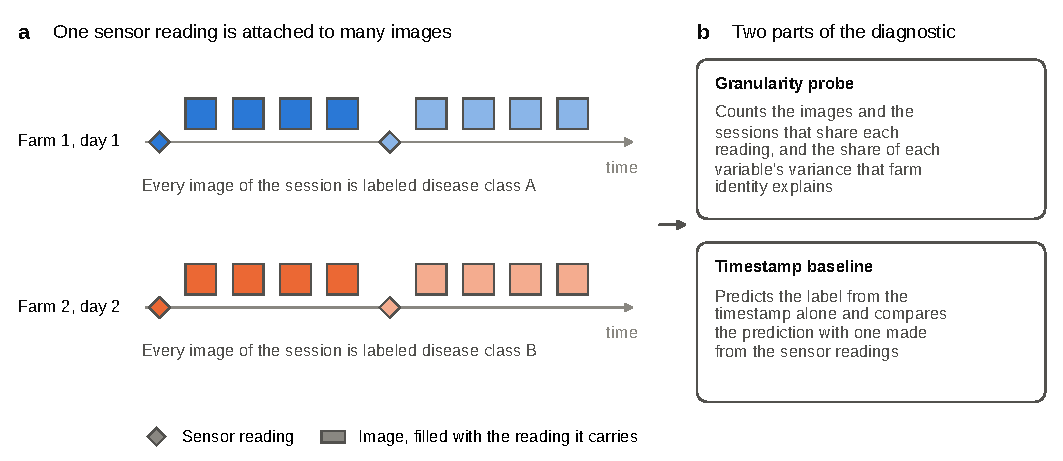
\includegraphics[width=\textwidth]{generated/fig_concept.pdf}
\end{center}
\caption{How one sensor reading is attached to many images, and the two parts of
the diagnostic. (a) A schematic of two sessions, each one farm on one day.
Each sensor reading (diamond) is attached to every image (square) taken after it
until the next reading, so the images of a session share far fewer readings than
there are images. (b) The two parts of the diagnostic. Neither part reads
an image.}
\label{fig:concept}
\end{figure}

We apply the diagnostic to the AI Hub and CDD datasets and re-analyze the CDD study
\citep{appliedsci2024dacon} on the split that it used, because the CDD study is the
only fusion study that we cite whose dataset and split were both released. We also
train the CDD study's fusion model on the AI Hub dataset on a split that holds out
whole photo dates. Most images of the AI Hub dataset were photographed on the day on
which their panel was measured, so such a split keeps the session of most test images
out of training. Such a split also keeps every class in both the training and the test data, so the
model is scored only on classes that it saw in training, whereas no split of CDD by photo
date does so, because some CDD classes were photographed on a single date. This paper has seven objectives: (1) to count, in both datasets, the images that share each
sensor reading; (2) to compare, on the AI Hub dataset, a classifier given only the
timestamp with one given the soil-chemistry readings; (3) to compare, on the same dataset, a classifier given the farm and the timestamp, which together identify the session, with one given every
recorded sensor variable; (4) to measure, within single sessions of the AI Hub dataset, the readings'
advantage over a majority-class predictor, which always outputs the most frequent
class; (5) to measure that advantage on CDD environment series held out of training;
(6) to score a classifier given only the timestamp on the CDD
study's own split, beside the macro-F1 that the study reports for its fusion model; and (7) to test whether the gain of the CDD study's fusion model on the AI Hub dataset is
smaller on a split that holds out whole photo dates than on a random split.

% ===========================================================================
\section{Materials and methods}
\label{sec:methods}

\subsection{Datasets}
\label{sec:corpora}

The Domestically Cultivated Subtropical and Tropical Pest and Disease Data
\citep{aihub2023subtropical}, the AI Hub dataset throughout this paper, is
distributed through AI Hub as a Training set and a Validation set, without a test
set, so we pool the two sets and draw every split that we use from them. The AI Hub
dataset's metadata spreadsheet holds \numImages{} rows, each naming one image file whose name
encodes the image's crop, plant part, and class. Each row also gives the farm, the
date and time at which the image was photographed, a soil and ambient panel (air
temperature, air humidity, soil moisture, soil temperature, soil pH, nitrogen,
phosphorus, potassium, and electrical conductivity), and the date and time at which
the panel was measured, although a row can lack some of the panel's values. The rows
span \numClasses{} pest and disease classes and a healthy class across
\numCrops{} crops: apple mango, banana, dragon fruit, fig, Hallabong mandarin,
lemon, olive, and passion fruit. We predict one
class per image and take the class from the image's file name. A usage guideline
that accompanies the dataset \citep{aihub2023subtropical} records that the environmental sensors
were installed per farm, at each of the \numFarms{} farms where the images were taken in
\photoWindow{}, and that the sensors' readings were matched to the images afterwards. For
\pctPhotoDayDiffers{}\% of the rows, the panel was measured on another day than the
one on which the image was photographed. We take the day of a row's session to be the
day on which its panel was measured, because a reading can identify only the session
in which it was measured.

The Crop Disease Diagnosis dataset \citep[CDD;][]{dacon2021cropdisease}, released
by LG AI Research through the Dacon challenge platform, pairs each of its
\cddImages{} labeled images of \cddCrops{} greenhouse crops with an annotation file
and an environment series, a time series of greenhouse sensor readings. The
annotation gives the date and time of the photograph and the image's crop, disease, and
disease severity. Each combination of crop, disease, and severity in the dataset is
one of \cddClasses{} classes. The images of
\cddSingleDateClasses{} of these classes were all photographed on a single date, so no
split by photo date keeps every class of CDD in both the training and the test data.

In both datasets, we leave the sensor values as they stand in the files, including the
AI Hub dataset's pH values outside the pH scale and its nitrogen, phosphorus, and
potassium values of exactly zero, because those are the values that a model trained on
either dataset receives.

\subsection{Granularity probe}
\label{sec:diagnostic}

The granularity probe tests whether each reading is shared by many images and whether
the readings vary mostly between farms, as readings that identify the session would.
On the AI Hub dataset, the share of a panel variable's variance that farm identity
explains is $\eta^2$ of a one-way analysis of variance with farm as the factor, which is
the between-farm sum of squares divided by the total sum of squares. A variable varies
mostly between farms if farm identity explains more than half of its variance, and
because sessions nest within farms, it then varies mostly between sessions as well.
Two rows share a reading when their panel tuples, the nine values of their readings, are
equal value by value, an empty value matching only an empty value. We counted the distinct panel tuples, the
percentage of rows that share their panel tuple with at least one other row, and the
number of panel tuples that occur in only one session. CDD stores each image's
environment series in a CSV file of its own and stamps each row of the series with
its reading time, so the files of two images can differ in their stamps alone. We
therefore treated two images as carrying the same environment series when their files
hold identical values once the column of reading times is dropped. CDD names no
greenhouse, so on CDD the images that share one series approximate a session. We
counted the distinct series and the percentage of images that share their series with
another image. To test whether a series identifies one day and one disease, we took
the series that more than one image carries. We computed the percentage of them whose
images were all photographed on one date, and the percentage of them whose images all
carry one disease (the disease that an image's annotation records apart from the crop
and the severity).

\subsection{Timestamp baseline}
\label{sec:timestamp-methods}

The timestamp baseline compares random forests \citep{breiman2001random} from the
scikit-learn library \citep{pedregosa2011scikit} that read the sensor readings with
forests that read a timestamp, and sets beside them forests that read a timestamp
together with the farm or with the readings (Table~\ref{S-tab:settings} in the
supplementary data). On the AI Hub dataset, each forest was trained and
scored within a crop, because \numSingleCropClasses{} of the \numClasses{} pest and
disease classes occur on one crop only and could be predicted from the crop. A crop
enters the comparison if at least \timestampMinRows{} of its rows carry all five
soil-chemistry variables (pH, N, P, K, and electrical conductivity) and those rows span
at least two classes, which excludes only the Hallabong mandarin, for which the dataset records no potassium value. The soil-chemistry classifier reads the five soil-chemistry
variables, because they describe the soil's nutrient status, through which the readings could
carry agronomic information about disease. The full-panel classifier reads every panel variable recorded in the rows that carry
all five soil-chemistry variables. In every compared crop, these are the soil chemistry,
air temperature, air humidity, and soil temperature, and in apple mango, soil moisture
as well.  The timestamp
classifier reads the day and the time of day at which a row's panel was measured, and
the farm-and-timestamp classifier reads the same two values and the farm, which
together identify the session. Comparing the full-panel classifier with the
timestamp classifier shows whether the variables beyond soil chemistry change the result
of the soil-chemistry classifier's comparison with the timestamp classifier. A full-panel classifier that is more accurate than the farm-and-timestamp
classifier predicts more than the session alone would.

Each of the \timestampCrops{} compared crops has more than \timestampSampleRows{} rows
that carry all five soil-chemistry variables. To bound the computation, we drew
\timestampSampleRows{} of those rows at random in each crop and scored the four
classifiers on them by stratified \timestampFolds{}-fold cross-validation. Like a random split, this
cross-validation can place rows of one session in both the training and the test folds,
so a timestamp can predict the class by identifying the session. We repeated the
draw and the cross-validation for each of \numSeeds{} random seeds. Every classifier
used the same rows, folds, and seed. A majority-class predictor, which always predicts
the most frequent class of the training folds, was scored on the same folds. We scored accuracy and balanced accuracy, the mean over classes of the share of each
class's rows that the classifier assigns to that class. Comparing the two scores shows
whether a comparison depends on the sizes of the classes. A classifier's margin over another is
its accuracy or balanced accuracy minus the other's. We then repeated the
comparison with every forest tuned in an inner cross-validation within each set of
training folds, using the same grid search for every classifier (Table~\ref{S-tab:settings}).

If the soil-chemistry readings only identify the session, they should predict little
once the session is fixed. We therefore scored the soil-chemistry classifier, under each of the \numSeeds{} seeds, by
stratified \timestampFolds{}-fold cross-validation inside each session of at least \sessionMinRows{} rows (the session minimum) that holds
at least two classes each large enough to appear in every fold. For comparison, we also
pooled the rows of those sessions within each crop and scored the soil-chemistry classifier by one cross-validation over the pooled rows. The soil-chemistry classifier's advantage is its
margin in accuracy over the majority-class predictor. We averaged the advantage within each crop over its
sessions, weighting each session by its number of scored rows, and then over the crops
and the seeds.

On CDD, we drew two splits over \cddSeeds{} random seeds each. Under each seed, the
images are divided into \cddFolds{} folds, and one fold is held out for testing. The folds are stratified by class alone
(the random split) or also grouped by environment series, so that each series falls in
exactly one fold (the group-disjoint split, which approximates a session-disjoint
split). On CDD, untuned random forests like those
of the AI Hub comparison predict the \cddClasses{}-class label. The environment
classifier reads the environment features, which are the mean, minimum, maximum, and
first and last non-missing values of each column of the environment series. The timestamp
classifier reads the day and the time of
day of the photograph, which is the timestamp that CDD's annotation records, whereas
on the AI Hub dataset it is the time of the panel's measurement. The
timestamp-and-environment classifier reads both the timestamp and the environment
features, so it shows whether the environment features add to the timestamp. A majority-class predictor is scored
on the same test images.

\subsection{Re-analysis of a published fusion study on CDD}
\label{sec:reanalysis}

The CDD study \citep{appliedsci2024dacon} scores its classifiers by macro-F1, the
unweighted mean over classes of the F1 score, which for one class is the harmonic
mean of its precision and recall. The study reports that adding the environment
series to a ResNet-50 image classifier raises macro-F1 from \paperImageFone{} to
\paperMultiFone{} \citep[Table~2]{appliedsci2024dacon}. The study obtained both values
without its multimodal mixup augmentation, which adds training examples that blend
pairs of examples linearly in image and series. Our training of the study's fusion
model on the AI Hub dataset also leaves that augmentation out. The study states a ratio of training,
validation, and test images but not how it drew its split, so we took the split from
the study's public repository \citep{cropdiseaserepo}. The repository holds two sets of identifiers, each with a training, a validation, and a test partition. The study's
split is the set that the study's training script reads. We matched the identifiers
to the environment series, computed the share of test images whose series also occurs
in training (the leak rate), and counted the test identifiers that appear verbatim in
training. Table~\ref{S-tab:leak} gives the leak rates with series matched by their
raw files, reading times included, and the leak rates of the repository's other set of
identifiers.

We then ran the forests of the CDD timestamp baseline on the study's split, with its
identifiers unchanged, so that their macro-F1 and the study's are measured over the
same test images. These untuned forests select no hyperparameter, so they train on the
study's training and validation partitions together. However, a forest considers about
the square root
of the number of input variables at each node of a tree, so the
timestamp-and-environment classifier, whose two timestamp columns are far outnumbered by the environment features, rarely considers a timestamp column. For every classifier,
we therefore also chose the number of variables per node, from a grid of values that
includes the number of all input variables, by the macro-F1 that a forest trained on the study's training
partition reaches on the study's validation partition. We then trained a forest with
the chosen number on both partitions together (Table~\ref{S-tab:settings}). The comparison of the timestamp classifier alone with the macro-F1 that the study
reports for its fusion model was chosen after we had seen the scores of the timestamp, environment, and timestamp-and-environment classifiers and
of the majority-class predictor on the split. That comparison is therefore post hoc.

\subsection{Image--sensor fusion experiment on the AI Hub dataset}
\label{sec:fusion-design}

The fusion experiment trains the CDD study's fusion model on the AI Hub dataset and
holds out photo dates rather than farms, because a farm-disjoint split of the whole
metadata spreadsheet would leave \farmUncoveredPct{}\% of the test images with a
combination of crop, plant part, and class that no training image has, so the split would score the image-only and fusion models on kinds of image that their
training lacks. A split of the
spreadsheet by photo date, by contrast, leaves no test image with such a combination.
Only \candidateDateLeak{}\% of the test images of that split carry a panel tuple that
also occurs in training, so holding out photo dates also keeps the readings of most test images out
of training (Table~\ref{S-tab:candidates}). We drew a subsample of
\subsampleSize{} images stratified by crop, plant part, and class, to bound the
training cost, and split it two ways, each holding out one fold for testing: at random
(the in-distribution split) and by photo date (the date-disjoint split). The validation set, on which the epoch to keep is chosen, was drawn from the training
images by the same grouping as the test images.

The image-only model is a ResNet-50 \citep{he2016deep} pretrained on the ImageNet
image database \citep{deng2009imagenet} and taken from timm, a library of image
models \citep{wightman2019timm}. The fusion model is the late-fusion model that the
CDD study's repository releases \citep{cropdiseaserepo}, which combines the
ResNet-50's class scores with those of an environmental branch, a long short-term
memory (LSTM) network \citep{hochreiter1997lstm} followed by two fully connected
layers. The branch reads the panel as a sequence of length one, because an AI Hub
image carries one panel reading rather than a series. Both models follow the CDD
study's training procedure for its \matchedEpochs{} epochs (Table~\ref{S-tab:settings}), including its Adam optimizer \citep{kingma2015adam}, its learning-rate schedule \citep{loshchilov2017sgdr}, its choice of the epoch with
the best validation macro-F1, and its random transformations of the training images.
We trained each model with \fusionSeeds{} random seeds,
a number that bounds the training cost. Training first ran for a reduced budget of
\lowBudgetEpochs{} epochs, which showed no gain of the fusion model over the
image-only model on the in-distribution split (Table~\ref{S-tab:fusion-reduced}), and
then for the study's number of epochs. The in-distribution gain that we report
therefore comes from training runs that we added after a null result.

The image-only and fusion models share the ResNet-50, the training procedure, and the
random seeds, so
they differ only in the panel and in the layers that read it. The fusion gain
\begin{equation}
\delta = \mathrm{macroF1}(\text{image}+\text{panel}) - \mathrm{macroF1}(\text{image})
\label{eq:gain}
\end{equation}
is therefore what the panel contributes to macro-F1 through those layers, taken
within a seed. The in-distribution gain and the date-disjoint gain are $\delta$ on the
two splits. The loss of the gain on held-out dates, the paired reduction, is the
in-distribution gain minus the date-disjoint gain, also taken within a seed, because a
seed sets the same initial weights for the runs on both splits.

\subsection{Statistical analysis and software}
\label{sec:stats}

We report each score from a set of seeds as the mean over the seeds, and each
interval as a 95\% confidence interval from the $t$ distribution. Where two
classifiers are scored on the same test images, we take their difference within seed
and conclude that one score is higher only where the interval of the difference
excludes zero. When we count the crops in which one classifier is more accurate than
another, a crop counts only where its paired $t$-test over the seeds remains
significant at the \holmAlpha{} level after Holm's correction for testing
\timestampCrops{} crops \citep{holm1979simple}, which lowers the level that each test
must reach so that the tests together keep that level. Where two scores come from splits
whose test images differ, we conclude that one is lower only where its interval lies
entirely below the other's, except for the paired reduction of the fusion experiment,
whose two gains pair within seed. On a fixed split, such as the CDD study's split or either
split of the fusion experiment, the seeds change only the forest or the training, so
the interval carries no variance from the choice of test images. The analyses ran in
Python \pythonVersion{} with pandas \pandasVersion{}, scikit-learn \sklearnVersion{},
PyTorch \torchVersion{} \citep{paszke2019pytorch}, timm \timmVersion{}, and
Albumentations \albumentationsVersion{}, a library of image transformations
\citep{buslaev2020albumentations}.

% ===========================================================================
\section{Results}
\label{sec:results}

\subsection{One sensor reading is shared by many images in both datasets}
\label{sec:res-diagnostic}

On both datasets, one sensor reading is shared across many images, so the readings
describe groups of images rather than measuring each one. On the AI Hub dataset,
farm identity explains more than half the variance of every panel variable except
air humidity and electrical conductivity (Fig.~\ref{fig:granularity}a). It explains
between \rsqFarmLo{} and \rsqFarmHi{} of the variance of pH, N, P, and K, four of the
five soil-chemistry variables that the soil-chemistry classifier reads. The dataset carries
only \numPanelTuples{} distinct panel tuples across its \numImages{} metadata rows. Of
the rows, \pctPanelTupleShared{}\% share their panel tuple with at least one other row.
Of the panel tuples, \numTuplesOneSession{} occur in only one session, so nearly every
panel tuple identifies its session.

\begin{figure}[t]
\begin{center}
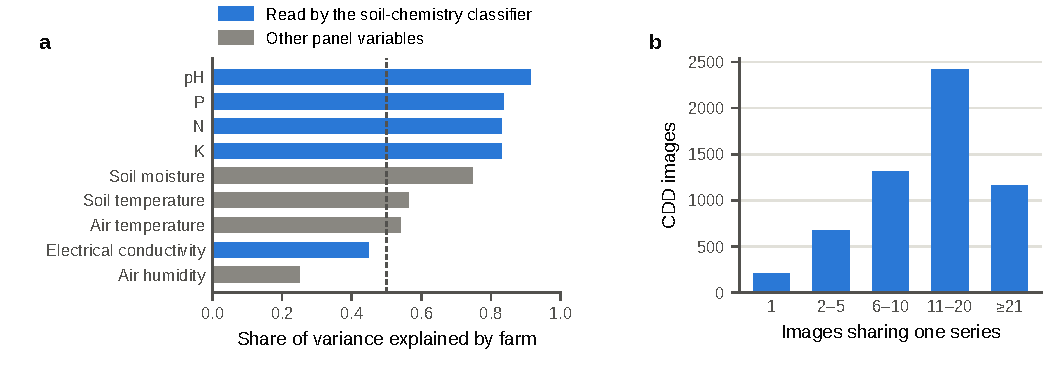
\includegraphics[width=\textwidth]{generated/fig_granularity.pdf}
\end{center}
\caption{Farm identity explains more than half the variance of every panel
variable of the AI Hub dataset except air humidity and electrical conductivity,
and most CDD images share their environment series with other images.
(a) The share of each panel variable's variance that farm identity
explains on the AI Hub dataset. The dashed line marks one half. The five soil-chemistry
variables that the soil-chemistry classifier reads are shown in blue.
(b) The CDD images grouped by how many images share their environment
series. A series shared by one image is a per-image reading.}
\label{fig:granularity}
\end{figure}

The granularity probe finds the same sharing on CDD. Only \cddSeries{} distinct
environment series exist for its \cddImages{} images. Of the images,
\cddSharedPct{}\% share their series with at least one other image
(Fig.~\ref{fig:granularity}b). Of the shared series, \cddSingleDatePct{}\% span a
single photo date and \cddSingleCodePct{}\% carry a single disease, so nearly every
shared series identifies one day, and nearly every one identifies one disease.

\subsection{A classifier given a timestamp is more accurate than one given the
soil-chemistry readings in \timestampHigherCrops{} of the \timestampCrops{} AI Hub
crops compared}
\label{sec:res-timestamp}

On the AI Hub dataset, the timestamp classifier is more accurate than the soil-chemistry
classifier in \timestampHigherCrops{} of the \timestampCrops{} crops
(Fig.~\ref{fig:timestamp}). Its margin is $\figWinPlain{}$ in fig and
$\mangoWinPlain{}$ in apple mango, and between $\timestampMarginSmallLo{}$ and
$\timestampMarginSmallHi{}$ in lemon, banana, and dragon fruit. In passion fruit, the
comparison detects no difference between the two classifiers, and in olive the soil-chemistry
classifier is more accurate, by \oliveLeanAbs{}. With tuned
forests, the timestamp classifier is more accurate than the soil-chemistry classifier in the
same five crops and less accurate in olive, and has the higher balanced accuracy in
the same five crops and the lower in olive (Table~\ref{S-tab:tuned}).
With untuned forests, the timestamp classifier has the higher balanced accuracy in
those five crops and in passion fruit, and the lower in olive (Table~\ref{S-tab:margins}). Both classifiers exceed the majority-class predictor in
every crop (Table~\ref{S-tab:scores}).

\begin{figure}[t]
\begin{center}
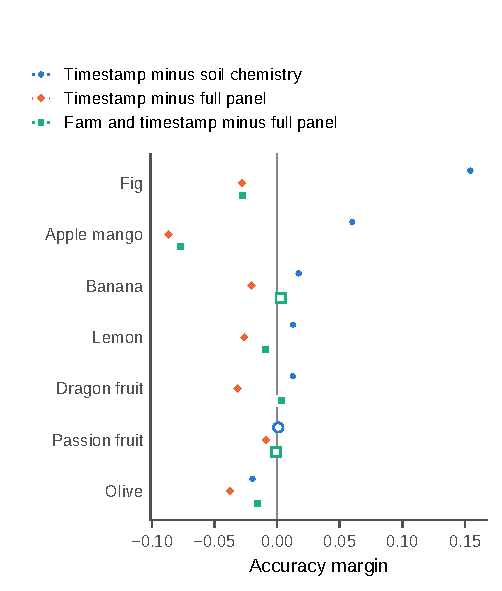
\includegraphics[width=0.5\textwidth]{generated/fig_timestamp.pdf}
\end{center}
\caption{Accuracy margins on the AI Hub dataset, per crop: the timestamp classifier
minus the soil-chemistry classifier, the timestamp classifier minus the full-panel classifier,
and the farm-and-timestamp classifier minus the full-panel classifier. Markers are
means over \numSeeds{} random seeds, and bars are 95\% confidence intervals. A marker
hides an interval narrower than itself. A hollow marker is a margin whose paired
$t$-test does not survive Holm's correction across the crops.}
\label{fig:timestamp}
\end{figure}

The full-panel classifier, by contrast, is more accurate than the timestamp
classifier in every compared crop, in both metrics and with the forests untuned or
tuned. Adding the farm to the timestamp removes the full-panel classifier's margin in banana
and passion fruit, where the full-panel and farm-and-timestamp classifiers do not differ. In dragon fruit, the
farm-and-timestamp classifier is the more accurate. In
the other \fullBeyondFarmCrops{} crops, lemon, fig, apple mango, and olive, the
full-panel classifier stays more accurate than the farm-and-timestamp classifier in
both metrics and with the forests untuned or tuned, by \fullBeyondFarmLo{} in lemon to
\fullBeyondFarmHi{} in apple mango in accuracy (Fig.~\ref{fig:timestamp}). One of these crops,
fig, has all its images from a single farm, so in fig this comparison adds nothing to the
comparison with the timestamp classifier.

\subsection{The readings lose part of their advantage within a session or on held-out
series}
\label{sec:res-within}

On the AI Hub dataset, the soil-chemistry classifier's advantage over the majority-class
predictor, averaged over the crops, falls from \panelAdvantagePooled{} with the
sessions pooled to \panelAdvantageWithinSession{} within single sessions. Each compared crop holds sessions that meet the session minimum of \sessionMinRows{}
rows, and in each crop the within-session advantage stays above
zero, between \residualLo{} and \residualHi{}. With a session minimum of \floorLow{} or \floorHigh{}
rows instead, the within-session advantage also stays above zero
in every compared crop (Table~\ref{S-tab:floors}).

On CDD, both the environment classifier and the timestamp classifier score a lower
macro-F1 on the group-disjoint split than on the random split (Table~\ref{tab:cdd}).
The environment classifier falls from \cddEnvRandom{} to \cddEnvGroup{} and the
timestamp classifier from \cddTimestampRandom{} to \cddTimestampGroup{}, so part of
each classifier's random-split score depends on series that training and test
images share. Neither classifier falls to the \cddBaseGroup{} that the majority-class
predictor scores on the group-disjoint split. The \cddSeries{} series spread over
\cddDates{} photo dates, an average of \cddSeriesPerDate{} series to a date, so a
held-out series leaves other series of its photo date in training. In macro-F1, the
timestamp and the environment classifiers do not differ on either split, whereas in
balanced accuracy the environment classifier scores higher on the group-disjoint split
(Table~\ref{tab:cdd}).

\begin{table}[t]
\centering
\footnotesize
\caption{Macro-F1 and balanced accuracy of the CDD predictors on the two splits
that we draw over the whole dataset, one random and one disjoint on the environment
series. Values are means over \cddSeeds{} random seeds with 95\% confidence
intervals. Each row is a random forest on the features that the row names, or the
majority-class predictor. A paired difference is the mean of the within-seed
differences, so it can differ in its last digit from the difference of the printed
means. The leak rate, a mean over the seeds without an interval, is the share of test
images whose environment series recurs in training.}
\label{tab:cdd}
\begin{tabular}{>{\raggedright\arraybackslash}p{0.30\textwidth}cc}
\toprule
 & Random split & Group-disjoint split \\
\midrule
\multicolumn{3}{l}{\emph{Macro-F1}} \\
Majority class & $\cddBaseRandom{}$~~$\cddBaseRandomCI{}$ & $\cddBaseGroup{}$~~$\cddBaseGroupCI{}$ \\
Environment & $\cddEnvRandom{}$~~$\cddEnvRandomCI{}$ & $\cddEnvGroup{}$~~$\cddEnvGroupCI{}$ \\
Timestamp & $\cddTimestampRandom{}$~~$\cddTimestampRandomCI{}$ & $\cddTimestampGroup{}$~~$\cddTimestampGroupCI{}$ \\
Timestamp and environment & $\cddTimestampEnvRandom{}$~~$\cddTimestampEnvRandomCI{}$ & $\cddTimestampEnvGroup{}$~~$\cddTimestampEnvGroupCI{}$ \\
\midrule
Timestamp minus environment & $\cddTimestampOverEnvRandom{}$~~$\cddTimestampOverEnvRandomCI{}$ & $\cddTimestampOverEnvGroup{}$~~$\cddTimestampOverEnvGroupCI{}$ \\
\midrule
\multicolumn{3}{l}{\emph{Balanced accuracy}} \\
Majority class & $\cddBaseRandomBA{}$~~$\cddBaseRandomBACI{}$ & $\cddBaseGroupBA{}$~~$\cddBaseGroupBACI{}$ \\
Environment & $\cddEnvRandomBA{}$~~$\cddEnvRandomBACI{}$ & $\cddEnvGroupBA{}$~~$\cddEnvGroupBACI{}$ \\
Timestamp & $\cddTimestampRandomBA{}$~~$\cddTimestampRandomBACI{}$ & $\cddTimestampGroupBA{}$~~$\cddTimestampGroupBACI{}$ \\
Timestamp and environment & $\cddTimestampEnvRandomBA{}$~~$\cddTimestampEnvRandomBACI{}$ & $\cddTimestampEnvGroupBA{}$~~$\cddTimestampEnvGroupBACI{}$ \\
Timestamp minus environment & $\cddTimestampOverEnvRandomBA{}$~~$\cddTimestampOverEnvRandomBACI{}$ & $\cddTimestampOverEnvGroupBA{}$~~$\cddTimestampOverEnvGroupBACI{}$ \\
\midrule
Leak rate (\%) & $\cddLeakRandom{}$ & $\cddLeakGroup{}$ \\
\bottomrule
\end{tabular}
\end{table}

\subsection{In the CDD study's split, \cddLeak{}\% of the test images share their
environment series with training images, and a timestamp classifier matches the
macro-F1 that the study reports for its fusion model}
\label{sec:res-cdd}

Images of the study's test partition recur in its training partition. Of its test
identifiers,
\cddDirectTest{}\% appear verbatim in its training partition and
\cddDirectTrainval{}\% in its training and validation partitions together, so the
study scores its models partly on images that they were trained on. For
\cddLeak{}\% of its test images, the identical environment series also occurs in
training. Of the \cddGroupsTotal{} distinct test series, \cddGroupsShared{} recur in
training, so the shared series are most of the test series, not a few series that
hold many test images. Our forests train on the training and validation partitions together, so the rate
relevant to them is the share of test images whose series occurs in either partition,
the leak rate into training and validation, \cddLeakTrainval{}\% (Table~\ref{tab:cdd-theirs}). The repository's other set of identifiers leaks too, so
neither shipped set is group-disjoint on the environment series (Table~\ref{S-tab:leak}).

\begin{table}[t]
\centering
\footnotesize
\caption{The predictors of Table~\ref{tab:cdd} scored on the CDD study's split, the
set of identifiers in the study's repository from which its training script reads
its training, validation, and test partitions. Scores are means over \cddTheirSeeds{}
random seeds of the forest, with 95\% confidence intervals, to four decimals, the
precision of the study's reported figures. The leak rate into training and validation, a
property of the split and therefore without an interval, is the share of test images
whose environment series occurs in either of those partitions. The paired difference is the mean of the
within-seed differences, so it can differ in its last digit from the difference of the
printed means.}
\label{tab:cdd-theirs}
\begin{tabular}{>{\raggedright\arraybackslash}p{0.26\textwidth}cc}
\toprule
 & Macro-F1 & Balanced accuracy \\
\midrule
Majority class & $\cddTheirBase{}$~~$\cddTheirBaseCI{}$ & $\cddTheirBaseBA{}$~~$\cddTheirBaseBACI{}$ \\
Environment & $\cddTheirEnv{}$~~$\cddTheirEnvCI{}$ & $\cddTheirEnvBA{}$~~$\cddTheirEnvBACI{}$ \\
Timestamp & $\cddTheirTimestamp{}$~~$\cddTheirTimestampCI{}$ & $\cddTheirTimestampBA{}$~~$\cddTheirTimestampBACI{}$ \\
Timestamp and environment & $\cddTheirTimestampEnv{}$~~$\cddTheirTimestampEnvCI{}$ & $\cddTheirTimestampEnvBA{}$~~$\cddTheirTimestampEnvBACI{}$ \\
\midrule
Timestamp minus timestamp and environment & $\cddTheirTimestampOverTimestampEnv{}$~~$\cddTheirTimestampOverTimestampEnvCI{}$ & $\cddTheirTimestampOverTimestampEnvBA{}$~~$\cddTheirTimestampOverTimestampEnvBACI{}$ \\
\midrule
Leak rate into training and validation (\%) & \multicolumn{2}{c}{$\cddLeakTrainval{}$} \\
\bottomrule
\end{tabular}
\end{table}

On the study's split, the timestamp classifier alone matches the macro-F1 that the
study reports for its fusion model, reaching \cddTheirTimestamp{} with an interval over
forest seeds that contains the study's \paperMultiFone{} (Table~\ref{tab:cdd-theirs};
Fig.~\ref{fig:cdd}). The timestamp-and-environment classifier reaches \cddTheirTimestampEnv{}. That score is above the \paperImageFone{} that the study
reports for its image model, below its fusion score, and below the timestamp alone. The timestamp alone also scores higher than the timestamp and the
environment features together when the number of variables per node is chosen on the
validation partition, and when a forest considers every variable at every node
(Table~\ref{S-tab:maxfeatures}). The environment features alone, without
the timestamp, reach \cddTheirEnv{}, far above the \cddTheirBase{} of the
majority-class predictor, so the environment classifier also predicts the class on
this split. On the repository's other set of identifiers, the timestamp
classifier also reaches the study's fusion score (Table~\ref{S-tab:other-set}).

\begin{figure}[t]
\begin{center}
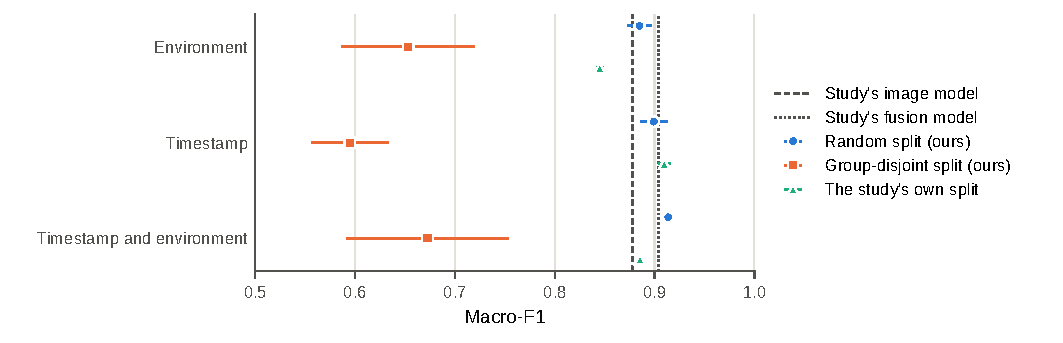
\includegraphics[width=\textwidth]{generated/fig_cdd.pdf}
\end{center}
\caption{Macro-F1 of three CDD predictors on the random and group-disjoint splits
that we draw and on the study's own split. Markers are means and bars are 95\%
confidence intervals. A marker hides an interval narrower than itself. The vertical
lines mark the macro-F1 that the study reports
for its image model and for its fusion model on its own split.
Tables~\ref{tab:cdd} and~\ref{tab:cdd-theirs} give the scores of the
majority-class predictor, which the figure omits.}
\label{fig:cdd}
\end{figure}

\subsection{A small late-fusion gain did not detectably shrink on held-out photo
dates}
\label{sec:fusion}

On the \subsampleSize{}-image subsample, a panel tuple that also occurs in training is
carried by \iidPanelLeak{}\% of the test images of the in-distribution split and by
\datePanelLeak{}\% of those of the date-disjoint split. The date-disjoint rate is close to the
\candidateDateLeak{}\% of the split of the whole spreadsheet by photo date. On
the in-distribution split, the fusion model raises macro-F1 relative to the image-only
model by $\delta = \iidDelta{}$ (Table~\ref{tab:fusion}). On that split, the image-only model's
macro-F1 after \matchedEpochs{} epochs minus its macro-F1 after the reduced-budget
training is $\imageOnlyBudgetChange{}$, and the fusion model's is
$\fusionBudgetChange{}$, so the in-distribution gain comes from a fall of the image-only model's score rather than from a rise of
the fusion model's (Table~\ref{S-tab:fusion-reduced}). On the date-disjoint split, the gain is
$\dateDelta{}$. The paired reduction of $\dateReduction{}$ is not detectably above
zero, so the date-disjoint split detects no loss of the gain on held-out dates. In
macro-F1, however, the date-disjoint gain itself is also not detectably above zero,
whereas in balanced accuracy it is.

\begin{table}[t]
\centering
\footnotesize
\caption{Late-fusion gain on the AI Hub dataset at the CDD study's training budget:
$\delta$ of Eq.~(\ref{eq:gain}), the fusion model's macro-F1 minus the image-only
model's, and the same difference in balanced accuracy. Values are
means over \fusionSeeds{} random seeds, with 95\% confidence intervals for the gains
and the reduction. The reduction is the in-distribution gain minus the date-disjoint
gain, paired within seed, so it can differ in its last digit from the difference of
the printed gains.}
\label{tab:fusion}
\begin{tabular}{lccc}
\toprule
 & Image-only macro-F1 & $\delta$, macro-F1 & $\delta$, balanced accuracy \\
\midrule
In distribution & $\imageOnlyFoneMatched{}$ & \stackci{$\iidDelta{}$}{$\iidDeltaCI{}$} & \stackci{$\iidDeltaBA{}$}{$\iidDeltaBACI{}$} \\
Date-disjoint & $\imageOnlyFoneDateMatched{}$ & \stackci{$\dateDelta{}$}{$\dateDeltaCI{}$} & \stackci{$\dateDeltaBA{}$}{$\dateDeltaBACI{}$} \\
Reduction & & \stackci{$\dateReduction{}$}{$\dateReductionCI{}$} & \stackci{$\dateReductionBA{}$}{$\dateReductionBACI{}$} \\
\bottomrule
\end{tabular}
\end{table}

% ===========================================================================
\section{Discussion}
\label{sec:discussion}

\subsection{What the sensor readings measure}

The fall of the soil-chemistry readings' advantage within a session shows that most
of their advantage on the AI Hub dataset comes from differences between sessions. On CDD, similarly, the photo date can account for the macro-F1 that the timestamp and
environment classifiers keep on held-out series (Section~\ref{sec:res-within}), because
the timestamp classifier reads the date and because environment series recorded on one
date can resemble each other, although in balanced accuracy the environment classifier
scores higher there. The readings
do more than identify the session, however, because the soil chemistry's advantage stays above zero within single
sessions (Section~\ref{sec:res-within}) and because, in \fullBeyondFarmCrops{} crops, the full-panel classifier is more
accurate than the farm-and-timestamp classifier, which reads what identifies the
session (Section~\ref{sec:res-timestamp}). Our
analyses do not show the source of the within-session advantage or of the full-panel classifier's
margin over the farm-and-timestamp classifier. Each could come from conditions that affect disease. Each could also come from conditions
that merely differed between the times at which the classes were photographed, because
a reading records such conditions and a timestamp does not.

Because the readings identify the session, a fusion model that relies on them can
lose the part of its gain that comes from session identity on farms or dates outside
its training data, provided that the classes differ between sessions. On the AI Hub
dataset, the in-distribution gain was itself small, \iidDeltaPoints{} percentage
points of macro-F1 against the \paperIncrement{} that the CDD study reports, so a loss
of a part of it on held-out dates may be too small to detect with \fusionSeeds{}
training runs per model.

\subsection{What the re-analysis of a published fusion gain can show}

On the published CDD split, a timestamp alone matches the macro-F1 that the CDD study
\citep{appliedsci2024dacon} reports for its fusion model, so nothing in the macro-F1
scores and intervals that the study publishes separates session identity from agronomic information in
the environment series. The CDD study reports confidence intervals from runs that vary
only the random seed of training on fixed split files \citep{appliedsci2024dacon}. A
leak raises the score but not the spread of the scores across runs, so a reader cannot
detect the leak from those intervals. A re-analysis can expose such a leak only where a study releases
both its dataset and its split, so our re-analysis covers one published gain.

\subsection{Recommendations for fusion studies and dataset releases}

A fusion study on a paired image--sensor dataset should report two things. The first is its fusion gain on a farm- or session-disjoint split, which keeps session
identity out of the gain whichever way the readings came to carry it. In the two datasets
here, the readings came to identify the session in two different
ways (Sections~\ref{sec:corpora} and~\ref{sec:diagnostic}): one panel reading attached to
many AI Hub images, and one CDD series repeated in many per-image files. A study
therefore cannot rule out session identity by checking for only one such way. The second is a sensor-only score, such as that of the soil-chemistry or environment
classifier here, set beside the scores of a majority-class predictor and
a timestamp classifier on the same test set and metric. A sensor-only accuracy far above the majority-class accuracy is not by itself evidence of agronomic
information, because session identity alone can produce it on a split that shares
sessions. Yet the fusion studies that we cite and that publish a sensor-only score
\citep{berrocal2026,agrifusion2026,jamun2025iot,cornsentry2026,appliedsci2024dacon,xu2025wheat}
set no majority-class score beside it, so a reader cannot tell how far those scores
exceed the majority-class score. \citet{berrocal2026}, for example, give their soil-moisture-only
baseline its own subsection and table, yet even they interpret that baseline's
accuracy as ``a meaningful but limited level of discrimination'' relative to their
image model rather than to a majority-class predictor.

Dataset releases can let readers check whether the sensor readings identify the
session before anyone trains a model. Two disclosures would tell a reader from the
release alone how many images share each sensor reading: the count of distinct sensor
readings and the unit over which a reading is constant, such as the session.

\subsection{Limitations}

Neither dataset has sensor readings that are known to carry agronomic information, so
we could not test whether the diagnostic distinguishes datasets whose readings identify
the session from datasets whose readings carry agronomic information. That test would
need a dataset that records a variable known to drive the disease at the plant and time
of each image. The diagnostic also cannot show that a dataset in which it finds no sign of session
identity is free of shortcuts, because a timestamp that fails to predict the class does not show
that the dataset holds no other input that predicts the class
\citep{feng2019misleading}. The timestamp baseline uses random
forests and the fusion experiment one late-fusion architecture, so neither sets an
upper bound on what another learner could extract from the readings. The
within-session advantage was measured for the soil-chemistry readings alone, so the full-panel classifier's advantage within single sessions is unmeasured. On CDD,
we scored no classifier on a split that holds out whole photo dates. Such a split would test whether the photo date accounts for the advantage of the CDD
classifiers over the majority-class predictor on held-out series, for
every class except the \cddSingleDateClasses{} that were photographed on a single
date. Both datasets
come from Korean farms and greenhouses, so the extent of session identity in the
readings of datasets collected elsewhere remains to be measured.

% ===========================================================================
\section{Conclusion}
\label{sec:conclusion}

Studies that fuse crop images with environmental sensor readings report gains on
paired datasets without establishing what the readings measure. A diagnostic that
reads no image shows that in both Korean datasets that we examined, nearly every image
shares its sensor reading with other images. A timestamp alone predicts the disease
class more accurately than the AI Hub dataset's soil-chemistry readings in most of
the crops compared. On the split of a published CDD fusion study, a timestamp alone
matches the fusion score that the study reports. The soil-chemistry readings lose
most of their advantage once the session is fixed, although the AI Hub dataset's
full panel predicts the class better than the farm and the timestamp together in
\fullBeyondFarmCrops{} of its \timestampCrops{} compared crops. A fusion study can
therefore show what its readings add to the image only on a split that keeps the
sessions of its test images out of training.

% ===========================================================================
\section*{CRediT authorship contribution statement}

Sungwoo Kang: Conceptualization, Methodology, Software, Formal analysis,
Investigation, Visualization, Writing -- original draft, Writing -- review \&
editing.

\section*{Declaration of generative AI and AI-assisted technologies in the writing process}

During the preparation of this work, the author used Claude (Anthropic) to assist
with code implementation as well as to improve the readability and language of the
manuscript. After using this tool, the author reviewed and edited the content as
needed and takes full responsibility for the content of the publication. The model
versions used were Claude Opus 4.8, Claude Opus 5, and Claude Opus 5.5.

\section*{Declaration of competing interest}

The author declares no known competing financial interests or personal relationships
that could have appeared to influence the work reported in this paper.

\section*{Acknowledgments}

We used the Domestically Cultivated Subtropical and Tropical Pest and Disease Data, a
dataset from The Open AI Dataset Project (AI Hub, S. Korea) built with
the support of the National Information Society Agency and funded by the Ministry of
Science and ICT. All information on this dataset can be accessed through AI Hub
(\url{https://www.aihub.or.kr}). This work received no funding.

\section*{Data availability}
\label{sec:availability}

The diagnostic and the fusion-analysis code are released with imagery-free
derived result tables in the GitHub repository
\url{https://github.com/hpicsk/session_confound}. Every measurement that we report
is read from these tables. Although the AI Hub dataset carries a
CC-BY-SA-4.0 label, we do not redistribute it, because its download channel is
restricted to approved domestic applicants. Its usage policy also forbids providing
the data to anyone whom its builders and the National Information Society Agency,
which supported its construction, have not approved.
Requests to access it should be directed to AI Hub \citep{aihub2023subtropical}.
The CDD dataset and the CDD study's code are not redistributed either. The values
that the CDD study reports are cited to the study rather than regenerated. For CDD,
our repository holds each image's identifier and two hashes of its environment series
(codes computed from the content, equal for equal content), one for each rule by which we match series: a hash of the raw CSV file and a hash of
its values once the column of reading times is dropped. Our repository holds none of CDD's images, sensor values, labels, crops, diseases, or photo dates and times,
which readers must obtain from Dacon \citep{dacon2021cropdisease}. For
both datasets, we release deterministic scripts that generate our splits rather
than frozen split indices, so a licensed holder regenerates identical splits.

\section*{Supplementary data}

Tables~\ref{S-tab:settings} to~\ref{S-tab:other-set} are in the supplementary data that
accompany this article.

\bibliographystyle{elsarticle-harv}
\bibliography{refs}

\end{document}
